\documentclass{standalone}
\usepackage{tikz}
\usetikzlibrary{shapes.geometric, arrows, positioning}

\begin{document}

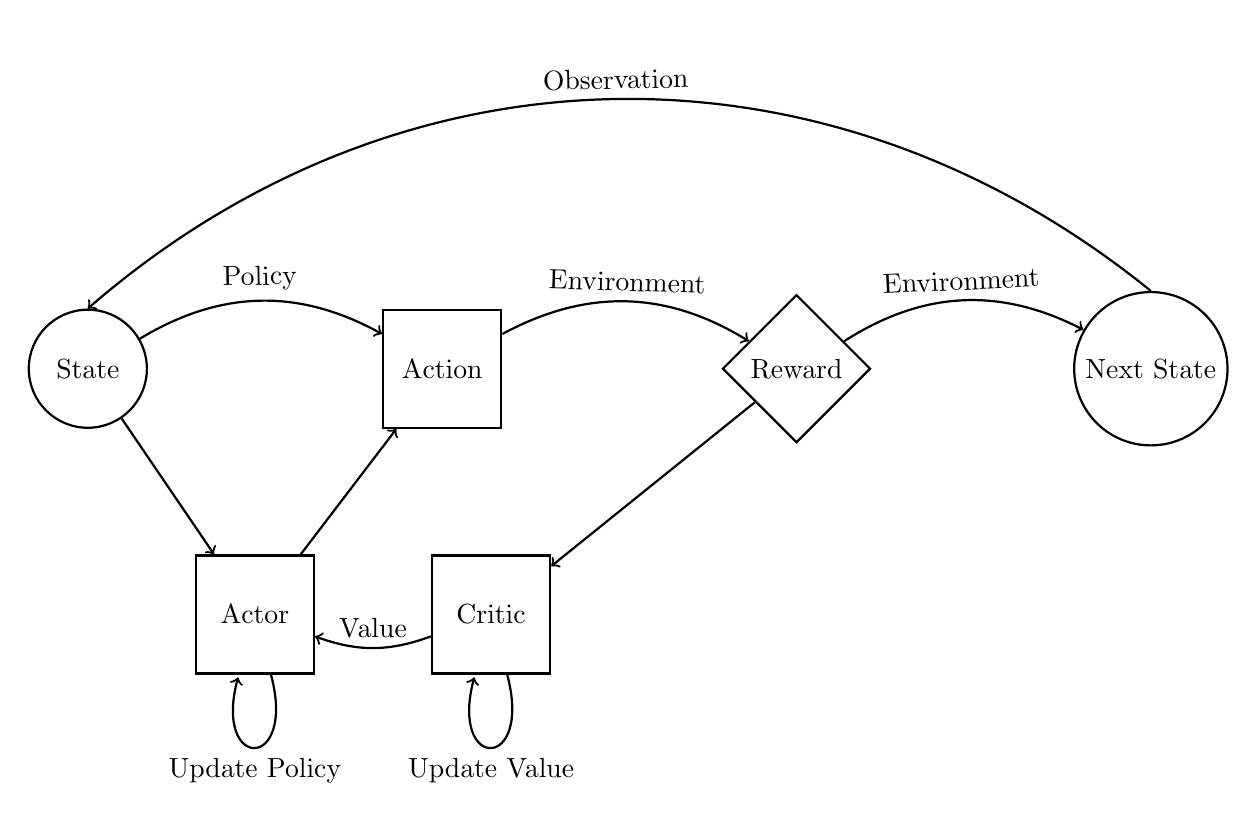
\begin{tikzpicture}[
    node distance=3cm,
    thick,
    state/.style={circle, draw, minimum size=1.5cm},
    action/.style={rectangle, draw, minimum size=1.5cm},
    reward/.style={diamond, draw, minimum size=1.5cm},
    actor/.style={rectangle, draw, minimum size=1.5cm, text centered},
    critic/.style={rectangle, draw, minimum size=1.5cm, text centered},
]

% Actor-Critic components
\node[actor] (actor) {Actor};
\node[critic, right of=actor] (critic) {Critic};

% Agent's environment interaction
\node[state, above left of=actor, yshift=1cm] (state) {State};
\node[action, right of=state, xshift=1.5cm] (action) {Action};
\node[reward, right of=action, xshift=1.5cm] (reward) {Reward};
\node[state, right of=reward, xshift=1.5cm] (next_state) {Next State};

% Arrows connecting the components
\path[->] (state) edge [bend left=30] node[above, sloped] {Policy} (action);
\path[->] (action) edge [bend left=30] node[above, sloped] {Environment} (reward);
\path[->] (reward) edge [bend left=30] node[above, sloped] {Environment} (next_state);
\path[->] (next_state.90) edge [bend right=40] node[above, sloped] {Observation} (state.90);

% Arrows connecting actor and critic
\path[->] (state) edge (actor);
\path[->] (actor) edge (action);
\path[->] (reward) edge (critic);
\path[->] (critic) edge [bend left=20] node[above, sloped] {Value} (actor);

% Data flow within the components
\path[->] (actor) edge [loop below] node[below] {Update Policy} (actor);
\path[->] (critic) edge [loop below] node[below] {Update Value} (critic);

\end{tikzpicture}

\end{document}
